\documentclass[a4paper,article,14pt]{extarticle}

\usepackage{spbudiploma}
\usepackage{amsmath}
\usepackage{mathtools}
\usepackage[pdftex]{graphicx}
\graphicspath{{../pictures/}}
\usepackage{listings}
\usepackage{xcolor}
\usepackage{amsfonts}


\usepackage{enumitem}
\definecolor{codegreen}{rgb}{0,0.6,0}
\definecolor{codegray}{rgb}{0.5,0.5,0.5}
\definecolor{codepurple}{rgb}{0.58,0,0.82}
\definecolor{backcolour}{rgb}{0.95,0.95,0.92}

\lstdefinestyle{mystyle}{
	backgroundcolor=\color{backcolour},   
	commentstyle=\color{codegreen},
	keywordstyle=\color{codegreen},
	numberstyle=\tiny\color{codegray},
	stringstyle=\color{codepurple},
	basicstyle=\ttfamily\footnotesize,
	breakatwhitespace=false,         
	breaklines=true,                 
	captionpos=b,                    
	keepspaces=false,                 
	numbers=left,                    
	numbersep=5pt,                  
	showspaces=false,                
	showstringspaces=false,
	showtabs=false,                  
	tabsize=2
}

\lstset{style=mystyle}

\begin{document}
	\begin{titlepage}
		\begin{center}
			FEDERAL STATE AUTONOMOUS EDUCATIONAL INSTITUTION
			
			OF HIGHER EDUCATION
			
			ITMO UNIVERSITY
			\vspace{3cm}
			
			\large\textbf{Report}
			
			\large on the practical task No. 3
			
			\large \flqq Algorithms for unconstrained nonlinear optimization. \\  First- and second-order methods\frqq
			\vspace{5cm}
			

			\begin{flushright}
				{Performed by:} \\
				Putnikov Semyon \\ 
				J4132c \\
			\end{flushright}
			
			
			\begin{flushright}
				{Accepted by:} \\
				Dr Petr Chunaev \\ 
			\end{flushright}
			\vfill
			
			{St. Petersburg}
			\par{\number\year}
		\end{center}
	\end{titlepage}

	\newpage
	
	\section{Goal}
	The use of first- and second-order methods (Gradient Descent, Conjugate Gradient Descent, Newton’s method and Levenberg-Marquardt algorithm) in the tasks of unconstrained nonlinear optimization.
	
	\section{Formulation of the problem}
	Generate random numbers $\alpha \in (0,1)$ and $\beta \in (0,1)$. Furthermore, generate the noisy data $\{x_k,y_k\}$, where $k = 0, \dotso, 100$, according to the following rule:
	$$y_k = \alpha x_k + \beta + \delta_k, \quad x_k = \frac{k}{100}$$
	where $\delta_k\: N(0,1)$ are values of a random variable with standard normal distribution. Approximate the data by the following linear and rational functions:
	\begin{enumerate}[label=(\arabic*)]
		\item $F(x,a,b) = ax + b$ \quad (linear approximant),
		\item $F(x,a,b) = \frac{a}{1+bx}$ \quad (rational approximant),
	\end{enumerate}
	by means of least squares through the numerical minimization (with precision $\varepsilon = 0.001$) of the following function: $$D(a,b) = \sum\limits_{k=0}^{100} (F(x_k,a,b)-y_k)^2$$
		
	To solve the minimization problem, use the methods of Gradient Descent, Conjugate Gradient Descent, Newton’s method and Levenberg-Marquardt algorithm. If necessary, set the initial approximations and other parameters of the methods. Visualize the data and the approximants obtained separately for each type of approximant. Analyze the results obtained (in terms of number of iterations, precision, number of function evaluations, etc.) and compare them with those from Task 2 for the same dataset.
	
	\section{Brief theoretical part}
	\subsection{Gradient Descent method}
	Gradient descent is based on the observation that if $f(x)$ is defined and differentiable in a neighbourhood of a point $a$, then $f(x)$ decreases fastest in a neighbourhood of $a$ in the direction of $-\nabla_{a}f$. One obtains the following formula: $$a_{n+1}=a_n - \gamma\nabla_{a_n}f$$ for $\gamma\in\mathbb{R}_+$ small enough, then $f(a_n) \geq f(a_{n+1})$. With this observation in mind, one starts with a guess $a_0$ for a local minimum of $f$, and considers the sequence $\{a_n\}$ such that $$a_{n+1}=a_n - \gamma\nabla_{a_n}f, n \geq 0$$
	Here the value of the step size $\gamma_n$ may be non-fixed and changed at every iteration (many possible ways to choose).
	
	\subsection{Conjugate Gradient Descent method}
	
	Given a function $f(x), x\in \mathbb{R}^n$ and an initial approximation $a_0$, one starts in the steepest descent direction: $$\Delta a_0=-\nabla_{a_0}f$$
	
	Find the step length $\alpha_0 := argmin_\beta f(a_0 +\alpha\Delta a_0)$ and the next point $a_1 = a_0 + \alpha\Delta a_0$. After this iteration, the following steps constitute one iteration of moving along a subsequent conjugate direction $s_n$, where $s_0 = \Delta a_0$:
	\begin{itemize}
		\item Calculate the steepest direction $\Delta a_n = -\nabla_{a_n}f$.
		\item Compute $\beta_n$ according to certain formulas.
		\item Update the conjugate direction $s_n = \Delta a_n + \beta_n s_{n-1}$.
		\item Find $\alpha_n = argmin_\alpha f(a_n + \alpha s_n)$.
		\item Update the position: $a_{n+1} = a_n + \alpha_n s_n$.
	\end{itemize}

	The choice of $\beta_n$ due to Fletcher-Reeves: $$\beta_n^{FR} = \frac{\Delta a_n^T \Delta a_n}{\Delta a_{n-1}^T \Delta a_{n-1}}$$
	
	The choice of $\beta_n$ due to Polak-Ribiere: $$\beta_n^{PR} = \frac{\Delta a_n^T (\Delta a_n - \Delta a_{n-1})}{\Delta a_{n-1}^T \Delta a_{n-1}}$$
	
	\subsection{Newton’s method}
	
	Let $f:\mathbb{R} \rightarrow \mathbb{R}$ be convex and twice-differentiable. Find the roots of $f'$ by constructing a sequence an from $a_n$ initial guess $a_0$ s.t. $a_n \rightarrow x^*$ as $n \rightarrow \infty$, where $f'(x^*) = 0$, i.e. $x^*$ is a stationary point of $f$.
	
	From the Taylor expansion of $f$ near $a_n$ (think that $x^* \approx a_n + \Delta a$), $$f(a_n + \Delta a) \approx T_f (\Delta a) := f(a_n) + f'(a_n)\Delta a +\frac{1}{2} f''(a_n)(\Delta a)^2$$
	
	Use this quadratic functions as approximants to $f$ in a neighbourhood of $a_n$ and find their minimum points (take into account that $f''(x) > 0$): $$0=\frac{dT_f (\Delta a)}{d \Delta a} = f'(a_n) + f''(a_n)\Delta a \Rightarrow \Delta a = - \frac{f'(a_n)}{f''(a_n)}$$
	
	Incrementing $a_n$ by this $\Delta a$ yields a point closer to $x^*$: $$a_{n+1}=a_n + \Delta a=a_n - \frac{f'(a_n)}{f''(a_n)}$$
	
	It is proved that for the chosen class of $f$, $a_n \rightarrow x^*$ as $n \rightarrow \infty$.
	
	\subsection{Levenberg-Marquardt algorithm}
	The application of LMA is the \textbf{least-squares curve fitting problem}: given a set $(x_i, y_i)_{i=1}^m$, find the parameters $\beta$ (column vector) of the model curve $f(x,\beta)$ so that the sum of the squares of the deviations $S(\beta)$ is minimized: $$arg\min_{\beta} S(\beta)\equiv arg\min_{\beta} \sum_{i=1}^{m}[y_i - f(x_i,\beta)]^2$$
	
	Start with an initial guess for $\beta$. In each iteration step, the parameter vector $\beta$ is replaced by a new estimate $\beta + \Delta \beta$. To determine $\Delta \beta$, the function $f(x_i,\beta + \Delta \beta)$ is approximated by its linearization: $$f(x_i, \beta + \Delta \beta) \approx f(x_i, \beta) + J_i \Delta\beta, J_i = (\nabla_{x_i}f(\beta))^T$$
	
	The sum $S(\beta)$ has its minimum at a zero gradient with respect to $\beta$. The above first-order approximation of $f(x_i, \beta + \Delta \beta)$ gives $$S(\beta + \Delta \beta) \approx \sum_{i=1}^{m} [y_i - f(x_i, \beta) - J_i\Delta \beta]^2$$ or in vector notation, $$S(\beta+ \Delta \beta)\approx[y - f(\beta)]^T [y-f(\beta)]-2[y-f(\beta)]^T J\Delta \beta + \Delta \beta^T J^T J \Delta \beta,$$ where $J$ is the Jacobian matrix, whose i-th row equals $J_i$ , and where $f(\beta)$ and $y$ are vectors with i-th component $f(x_i, \beta)$ and $y_i$ , respectively.
	
	Taking the derivative of $S (\beta + \Delta \beta)$ with respect to $\Delta \beta$ and setting to zero gives $$(J^T J) \Delta \beta = J^T [y - f(\beta)],$$ that is in fact a system of linear equations with respect to $\Delta \beta$.
	
	The system may be replaced by $$(J^T J + \lambda I) \Delta \beta = J^T [y-f(\beta)],$$ where \textbf{I} is the identity matrix, giving the increment $\Delta \beta$ to the estimated parameter vector $\beta$.
	
	\section{Results}
	%Present the results of solving the assigned problems, including graphs and tables, as well as a brief discussion of the results obtained (at most 4 pages)
	
	All results of calcutions we can see at Figures \ref{results}.
	\begin{figure}[h!]
		\centering
		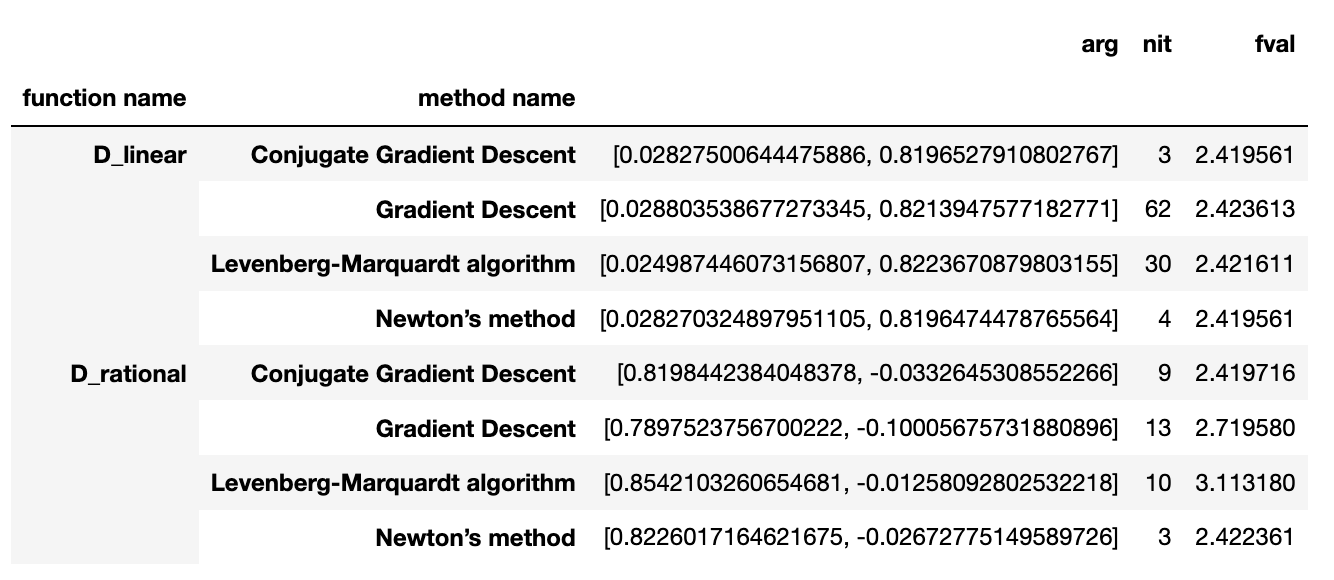
\includegraphics[scale=0.6]{results.png}
		\caption{Results of calcutions.}
		\label{results}
	\end{figure}
	
	\begin{figure}[h!]
		\centering
		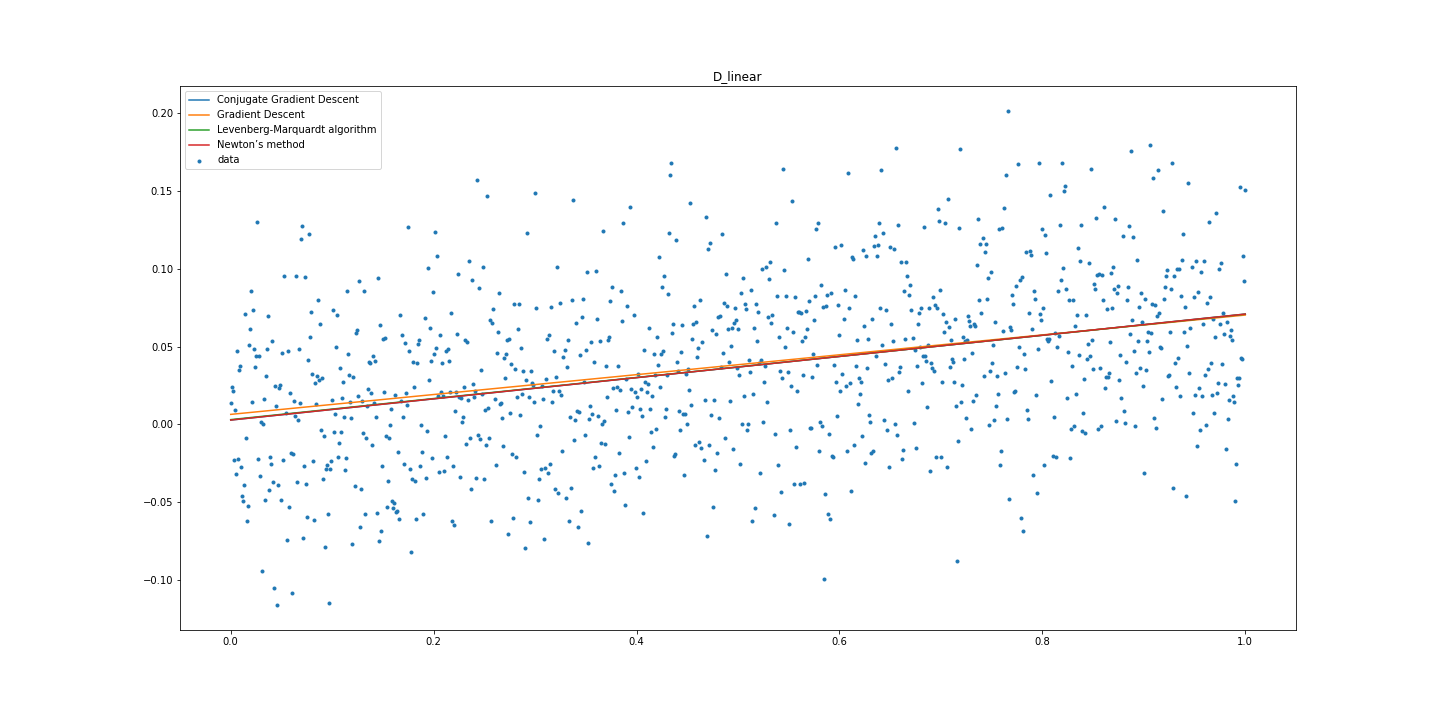
\includegraphics[scale=0.3]{D_linear.png}
		\caption{Linear approximant. Methods of Gradient Descent, Conjugate Gradient Descent, Newton’s method and Levenberg-Marquardt algorithm.}
		\label{linear}
	\end{figure} 
	
	\begin{figure}[h]
		\centering
		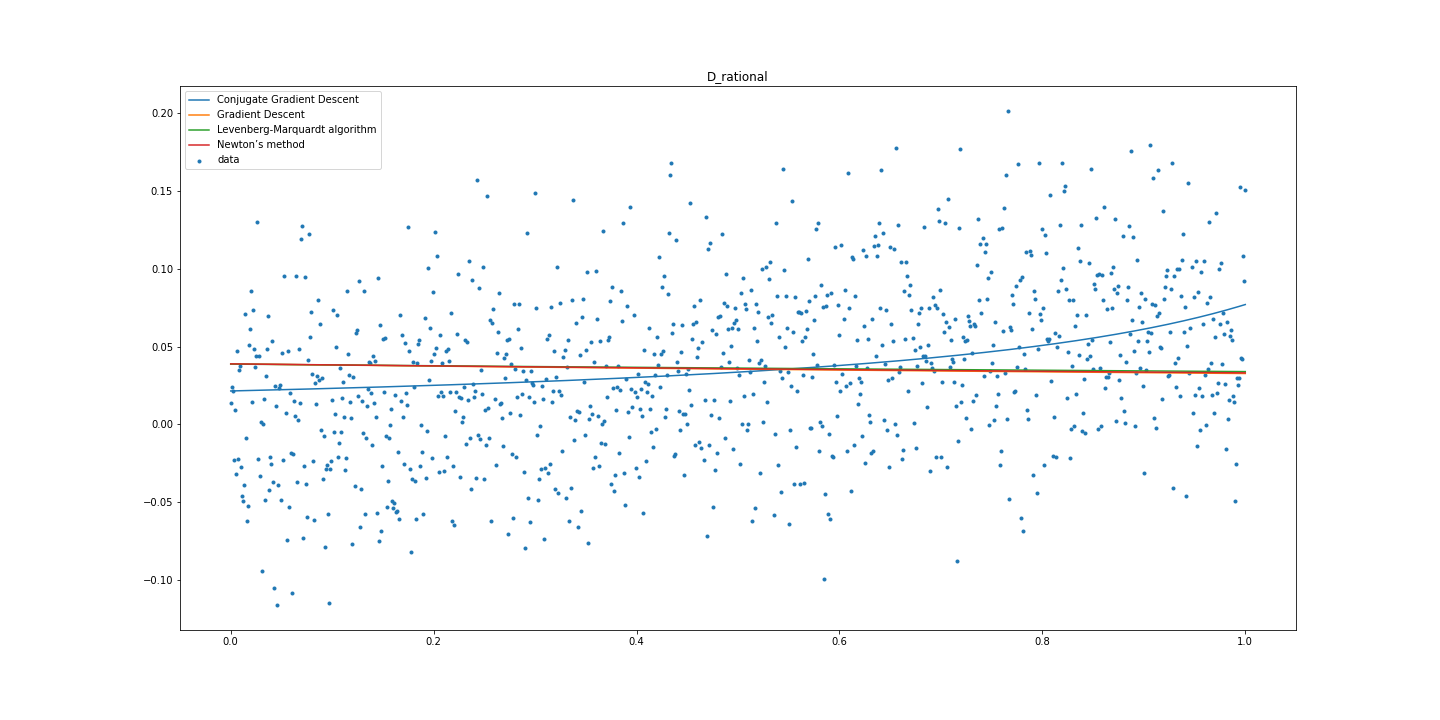
\includegraphics[scale=0.3]{D_rational.png}
		\caption{Rational approximant. Methods of Gradient Descent, Conjugate Gradient Descent, Newton’s method and Levenberg-Marquardt algorithm.}
		\label{rational}
	\end{figure} 
	
	All methods in case of liniar approximant (Figure \ref{linear})function converged to global minimum. Only one optimization method coverege to good approximation of rational approximant function (Figure \ref{rational}).
	
	Since the results of methods with linear function more representative, we can evaluate number of iterations. Most simplest method (Gradient Descent) worked for the greatest amount iterations. Newton and conjugate gradient methods are coverage with small number of iteration. Levenberg-Marquardt evaluate function more times than Newton or conjuate gradient method.
	
	If we will compare this results with results of second lab, we see that first- and second-order methods give better result with less amount of iterations.
	

	
\end{document}